\chapter{X/Motif Programs}
\label{chp:x-motif-programs}
This section describes the dialogs in the X/Motif programs \PrXmbtq{}, \PrXmbtr{} and \PrXmbtuser{},which are only briefly described in the user program list, together with \PrXmfilemon{}, the interface to the file monitoring tool.

\section{\XmbtqName{} - Optional Motif GUI Batch Queue Tool}
\PrXmbtq{} is a fully interactive Motif alternative to the standard batch queue manager, \PrBtq{}. As with
\PrBtq{} the format of the screen display, the help messages and even the command keystrokes can be easily altered to suit
your requirements.

Unlike \PrBtq{} there are no command line options to \PrXmbtq{}.

\subsection{Options}
It is not necessary to provide options via the resource files any more like with previous versions
of \PrXmbtq{} as the options selected within the program are automatically saved in the configuration
file \homeconfigpath{} off the user's home directory on request.

\subsection{The Main Window}
When \PrXmbtq{} is invoked the main window will be displayed. By default it will look something like this:

 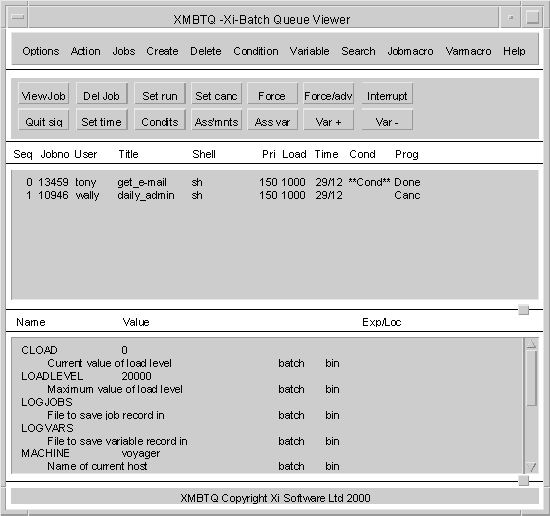
\includegraphics[width=14.399cm,height=13.653cm]{img/ref12.jpg} 

The main screen is divided into two key functional areas. The top area contains menus and short cut buttons for issuing commands. The bottom
area displays the batch jobs and variables, which may be selected to have commands performed upon them.

The key features of the batch jobs and variables area are:

 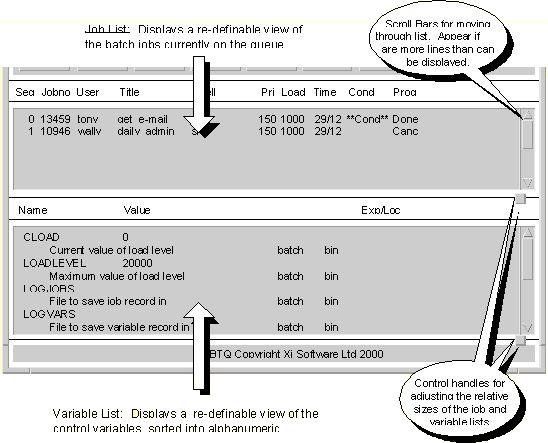
\includegraphics[width=14.346cm,height=11.718cm]{img/ref13.jpg} 

Variables and jobs can be operated upon by the appropriate menu options.
The job or variable must first be selected. This is done by clicking on
the line identifying it using the mouse. Once selected the line will be
highlighted.

If you cannot see the variable or job that you want then you may:

\begin{itemize}
\item Use the scroll bar or search menu options to find it.
\item Change the view to add the item or remove unwanted items from the display.
\end{itemize}
The key features of the top area are:

 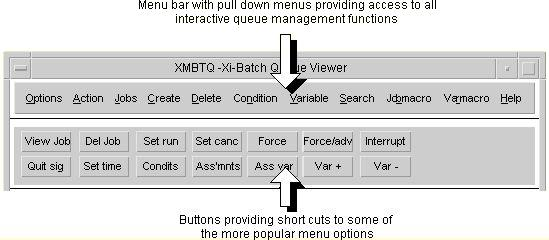
\includegraphics[width=14.376cm,height=6.346cm]{img/ref14.jpg} 

\subsection{The Menus and Shortcut Buttons}
All commands are performed by selecting a menu option or clicking on the equivalent shortcut button. Some of the menu options may also be
selected using shortcut keys, which are indicated to the right of the relevant options in each menu.

\subsubsection{The Options Menu}
 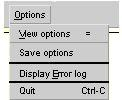
\includegraphics[width=3.193cm,height=2.646cm]{img/ref15.jpg} 

For tailoring the look and feel of \XmbtqName, saving the tailored settings, viewing the error log and quitting.

\textbf{View options} brings up the Display options dialog, to tailor the look and feel. Pressing the \exampletext{=} key also
invokes this option.

\textbf{Save options} saves the view options to the file \homeconfigpath{} in the user's home directory.

\textbf{Display Error log} brings up a Viewer showing any messages held in the \ProductName{} system log file, \filename{btsched\_reps}.

\subsubsection{The Action Menu \& Buttons}
 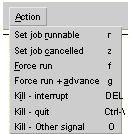
\includegraphics[width=3.454cm,height=3.544cm]{img/ref16.jpg} 

For high level actions: starting and stopping batch jobs.

\textbf{Set job runnable} will change a job from the Cancelled, Error or Abort state to the Ready or Run state. This option is also available
using the `\textbf{Set run}' shortcut button.

\textbf{Set job cancelled} puts a job on held (i.e. not able to run). This option is also available using the `\textbf{Set canc}' shortcut button.

\textbf{Force run} sets a job runnable and overrides any time specification to allow the job to run as soon as any Variable
Conditions are satisfied. This option is also available using the `\textbf{Force}' shortcut button.

\textbf{Force run + advance} sets a job runnable overriding any time specification to allow the job to run as soon as any Variable
Conditions are satisfied. The repeat time on the job is advanced to the next repetition. This option is also available using the
`\textbf{Force/adv}' shortcut button.

\textbf{Kill - interrupt} attempt to terminate a running job by sending it an Interrupt Signal. This option is also available using the
`\textbf{Interrupt}' shortcut button.

\textbf{Kill - quit} attempt to terminate a running job by sending it a Quit Signal. This option is also available using the
`\textbf{Quit sig}' shortcut button.

\textbf{Kill - Other signal} attempts to terminate a running job by sending it a specified Signal. This option opens a selection dialog.

\subsubsection{The Jobs Menu \& Buttons}
 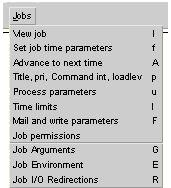
\includegraphics[width=4.479cm,height=4.971cm]{img/ref17.jpg} 

Provides options for inspecting and managing batch jobs which are currently visible in the job list.

\textbf{View job} opens a text browser showing the job script to be output. This option is also available using the `View job' shortcut button.

\textbf{Set job time parameters} brings up a dialog for setting the start time, retention options, repetition details and list of days to
avoid. This option is also available using the `Set time' shortcut button.

\textbf{Advance to next time} skips the next scheduled execution of a job by advancing to the next repetition.

\textbf{Title, pri, Command int, loadlev} opens the dialogue for setting the Title, Priority, Command Interpreter, and load level for the job.

\textbf{Process parameters} brings up the dialog to select the process parameters: working directory, ulimit, umask, network scope and which
exit codes represent an error.

\textbf{Time limits} opens the dialog for specifying time restrictions to terminate a runaway job.

\textbf{Mail and write markers} opens the dialog to specify what notification is required when a job finishes.

\textbf{Job permissions} brings up the dialog to set the access modes for the selected job.

\textbf{Job Arguments} opens a dialog for adding, editing and deleting arguments that are passed to the job on its command line.

\textbf{Job Environment} opens the dialog for adding, modifying and deleting the environment variables that are set up in the jobs run time
environment.

\textbf{Job I/O Redirections} opens the dialog for adding, editing and deleting I/O redirections.

\subsubsection{The Create Menu}
 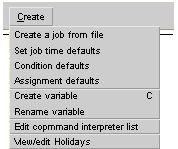
\includegraphics[width=4.657cm,height=3.941cm]{img/ref18.jpg} 

Provides options for Creating variables, requeueing jobs and setting up defaults.

\textbf{Create a job from file} opens a dialog to requeue a job that was earlier unqueued and perhaps modified. The dialog requires the name of
the command file of the unqueued job.

\textbf{Set job time defaults} sets default values for the set time dialog. These defaults are used when a job with no time, first has a
time set.

\textbf{Condition defaults} sets up a default pre-condition for editing the pre-conditions on jobs which so far have none.

\textbf{Assignment defaults} sets up a default assignment for editing the assignments on jobs which so far have none.

\textbf{Create Variable} brings up a dialog to create a new variable, including setting up the name, initial contents and comment.

\textbf{Rename Variable} changes the name of a variable, including all references to it in the pre-conditions and assignments of batch jobs.

\textbf{Edit command interpreter list} brings up the dialog for adding, changing and deleting command interpreters.

\textbf{View/edit Holidays} brings up the dialog for viewing and changing the holiday calendar.

\subsubsection{The Delete Menu}
 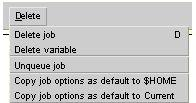
\includegraphics[width=5.129cm,height=2.722cm]{img/ref19.jpg} 

Contains options to unqueue jobs, delete jobs and deletes variables.

\textbf{Delete job} removes the selected job from the queue, provided it is not running. An error message is produced and the delete command
ignored if the job is running or the user does not have suitable
permission.

\textbf{Delete variable} removes the selected variable from the scheduler, providing no jobs specify it in a condition or assignment.
An error message is produced and the delete command ignored if the variable can be identified as in use or the user does not have suitable
permission.

\textbf{Unqueue job} opens the dialog to unqueue a copy of the selected job. The job may be deleted or not as required.

\textbf{Copy job options as default to \$HOME} takes the options from the selected job and saves them in a \filename{BTR}
environment variable in a file \homeconfigpath{} off the user's home directory.

\textbf{Copy job options as default to Current} takes the options from
the selected job and saves them in a \filename{BTR}
environment variable in a \configurationfile{} file in the
user's current directory.

\subsubsection{The Condition Menu}
 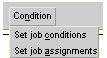
\includegraphics[width=2.798cm,height=1.535cm]{img/ref20.jpg} 

Provides options for setting up pre-conditions and assignments.

\textbf{Set job conditions} brings up the dialog to add, modify and
delete pre-conditions on the selected batch job.

\textbf{Set job assignments} brings up the dialog to add, modify and
delete assignments for the selected batch job.

\subsubsection{The Variable Menu}
 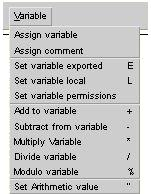
\includegraphics[width=3.955cm,height=5.129cm]{img/ref21.jpg} 

Provides options for manipulating variables.

\textbf{Assign variable} brings up the dialog to modify the data held by
the selected variable.

\textbf{Assign comment} brings up the dialog to modify the comment field
of the selected variable.

\textbf{Set variable Exported} makes the variable accessible by all
co-operating \ProductName{} hosts.

\textbf{Set variable Local} restricts access to the variable to the
local machine.

\textbf{Set variable permissions} brings up the dialog to modify the
access modes for the selected variable.

\textbf{Add to variable} increments the value of the selected variable
by the currently set Arithmetic Value.

\textbf{Subtract from variable} decrements the value of the selected
variable by the currently set Arithmetic Value.

\textbf{Multiply variable} multiplies the value of the selected variable
by the currently set Arithmetic Value.

\textbf{Divide variable} divides the value of the selected variable by
the currently set Arithmetic Value.

\textbf{Modulo variable} performs a modulo on the value of the selected
variable by the currently set Arithmetic Value.

\textbf{Set arithmetic value} for the above operations.

\subsubsection{The Search Menu}
 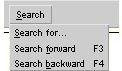
\includegraphics[width=3.193cm,height=1.879cm]{img/ref22.jpg} 

Both the variable and job lists may be navigated by using search options
to find items of interest.

\textbf{Search for} selected item or pattern.

\textbf{Search forward} from the current position

\textbf{Search backward} from the current position

\subsubsection{The Jobmacro Menu}
 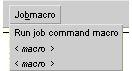
\includegraphics[width=3.454cm,height=1.879cm]{img/ref23.jpg} 

Provides options for running macro commands related to the selected
batch job.

\textbf{Run job command macro} opens a dialog prompting for the name of
the macro to run. This is then invoked by \XmbtqName{} with the job id number
of the selected job.

\textbf{{\textless}}\textbf{\textit{macro}}\textbf{{\textgreater}} runs
the pre-defined macro, whose name or a brief description will appear in
place of the {\textless}\textit{macro} {\textgreater} place holder.

Up to 9 macros may be pre-defined.

\subsubsection[The Varmacro Menu]{The Varmacro Menu}
 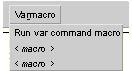
\includegraphics[width=3.454cm,height=1.879cm]{img/ref24.jpg} 

Provides options for running macro commands related to the selected job control variable.

\textbf{Run var command macro} opens a dialog prompting for the name of the macro to run. This is then invoked by \PrXmbtq{}
and passed the name of the selected variable.

\textbf{{\textless}}\textbf{\textit{macro}}\textbf{{\textgreater}} runs the pre-defined macro, whose name or a brief description will appear in
place of the {\textless}\textit{macro}{\textgreater} place holder.

Up to 9 macros may be pre-defined.

\subsubsection{Help}
 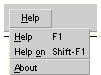
\includegraphics[width=2.641cm,height=1.983cm]{img/ref25.jpg} 

Context sensitive help for using \PrXmbtq{}.

\textbf{Help} displays help for the current window.

\textbf{Help on} changes the operating mode from taking commands to displaying help on any object (menu, button etc) that is selected.

\textbf{About} displays information, such as release number, about the version of \PrXmbtq{} that is running.

\subsection{Setting the View Options}
The content and format of information displayed by \XmbtqName{} can be customised via the \textbf{View options} item under the Options menu.
Confirmation for the delete commands may also be set under this option.

Selecting this option opens the following dialog window.

 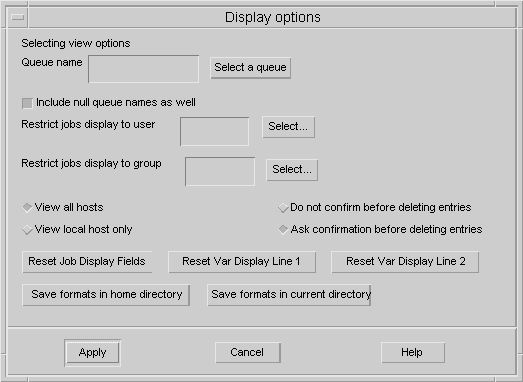
\includegraphics[width=13.695cm,height=10.104cm]{img/ref26.jpg} 

\subsubsection{Setting the Confirmation level}
 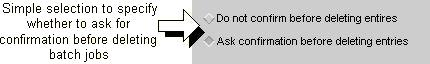
\includegraphics[width=11.261cm,height=1.692cm]{img/ref27.jpg} 

By default \PrXmbtq{} asks for confirmation before deleting any job from the queue. This may be relaxed to allow jobs to
be deleted without confirmation.

\subsubsection{Restricting the display}
The display may be restricted by effectively filtering to only show information for selected users, groups, job queues and local or all
\ProductName{} hosts.

\paragraph{Restricting the display to the local host}
 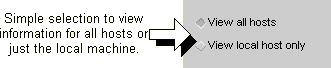
\includegraphics[width=8.668cm,height=1.796cm]{img/ref28.jpg} 

All hosts running \ProductName{} in the networked mode can be treated as a single system. By default \XmbtqName{} will show all of the externally visible
jobs and variables. The view can be restricted to show just the local job queue and variables.

\paragraph{Restricting the display by job queue}
The job display can be restricted by selecting a set of job queue names or patterns matching job queues.

 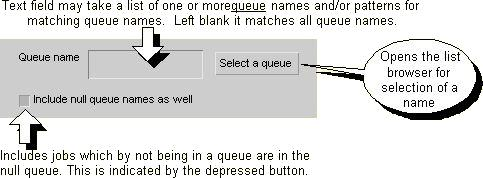
\includegraphics[width=12.644cm,height=4.71cm]{img/ref29.jpg} 

\paragraph{Restricting the display by user \& group}
The display may be restricted to jobs and variables owned by a specified user or set of users. Similarly to users it may be restricted to one or
more primary groups.

 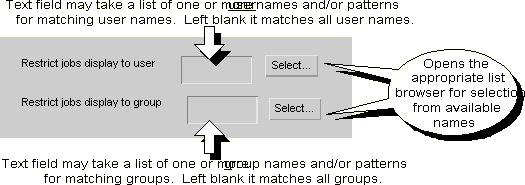
\includegraphics[width=13.748cm,height=4.895cm]{img/ref30.jpg} 

Sets of users or groups may contain just one name, a list of names or a list of patterns for matching names. The group and user names may be
given as a comma-separated list of alternatives, including the use of shell-style wild-cards. For example

\begin{expara}

fred

jmc,tony,ukops\_jmc,ukops\_wal

ukops*,ukadmin[1-5]

[m-z]*

\end{expara}

The wild-card options are:

\begin{center}
\begin{tabular}{ll}
\exampletext{*} & Matches anything\\
\exampletext{?} & Matches one character\\
\exampletext{[a-m]} & Matches one character in list or range\\
\exampletext{[!n-z]} & Matches one char not in list or range\\
\end{tabular}
\end{center}

\subsubsection{Changing the fields displayed and their format}
There is far more information available for both jobs and variables than could be displayed in the main window of \PrXmbtq{}.
Different columns of information may be displayed as required. The field widths and handling of field overflow may also be adjusted.

For example: If your batch jobs often have arguments and long titles, and you do not need the shell column in the job display, then you could
do the following:

\begin{itemize}
\item Delete the shell column.
\item Make your \PrXmbtq{} main window wider by dragging it with the mouse.
\item Add a job argument column.
\item Increase the Title width from 13 to say 25 characters.
\end{itemize}
To edit the job or variable displays click on the appropriate button:

 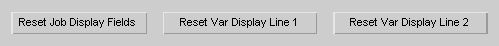
\includegraphics[width=13.063cm,height=1.214cm]{img/ref31.jpg} 

The variable display uses two lines for each variable, which are edited separately, hence the separate buttons for editing each line.

\paragraph{Changing the Job Display}
Clicking on the Reset Job Display Fields brings up the following window. The row of buttons at the top are for adding, changing and deleting
fields or separators. The fields are the columns of information and the separators are the column dividers.

 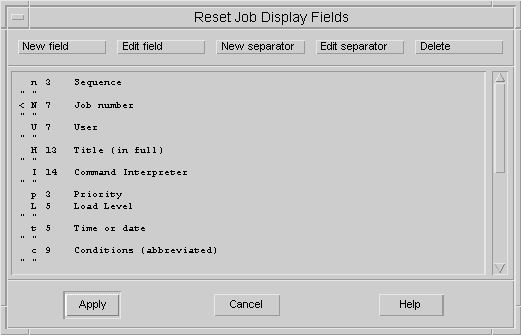
\includegraphics[width=13.638cm,height=8.864cm]{img/ref32.jpg} 

Underneath the row of buttons is a scrollable text window showing the display format. Each line holds the specification for one column or
column divider, as follows:

 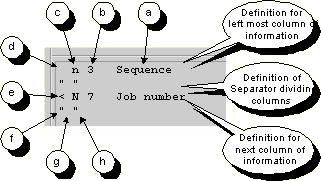
\includegraphics[width=8.401cm,height=4.785cm]{img/ref33.jpg} 

\begin{enumerate}
\item Field description / title
\item Width in characters
\item Field Identifier
\item No action on field overflow
\item Overflow onto left hand field is permitted
\item Open quote before separator
\item Separator character(s)
\item Close quote after separator
\end{enumerate}
To edit an existing field select the line showing the specification for that field and click on the Edit field button. To insert a new field
select the line underneath the point at which you want to insert it and click on the New field button. Either of these actions will bring up a
``Job display field'' window looking something like this:

 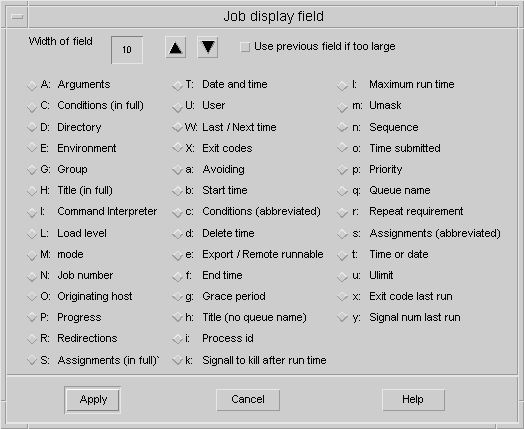
\includegraphics[width=13.72cm,height=11.351cm]{img/ref34.jpg} 

The width of field can be adjusted by typing in a new value or using the up and down arrow buttons. The ``Use previous
field...'' button is to allow a field to overflow into the field on its left. Pressing the button changes it from the deselected
to selected state and vice versa.

The other buttons allow selection of what information will be displayed in the column. Only one of these buttons may ever be in the selected
state. When a button is selected the field width is reset to a suitable value for the data to be displayed. This value may then be adjusted as
required.

\paragraph{Changing the Variable Display}
The principles for the variable display are almost the same as those for the job display. The only difference is that each variable is listed on
two lines, the format of which are edited separately. Similar windows are used, only the display information inside is different.

\subsubsection{Saving the Format Changes}
These are saved by assignments to an appropriately-named variable in \homeconfigpath{} off the user's home directory or in \configurationfile{}
in the current directory.

(Note that the whole help file is no longer copied).

\subsubsection{Saving the View Options}
All of the view options are saved on request using keywords in the \homeconfigpath{} file off the user's home directory.

\PrXmbtq{} no longer saves local copies of the resource file as was done in previous versions.

\subsection{Viewing a Batch Job}
Selecting a batch job from the display then selecting the \textbf{View job} option from the \textbf{Jobs} menu opens this window.

 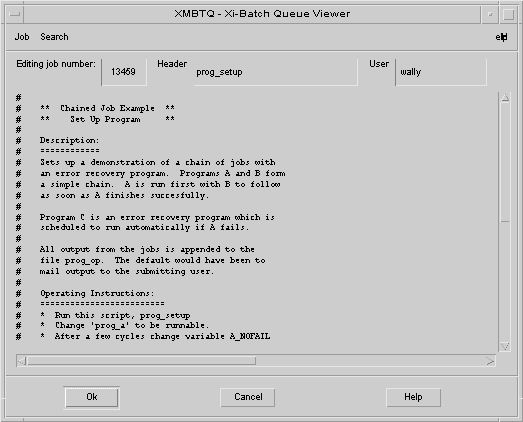
\includegraphics[width=13.695cm,height=11.164cm]{img/ref35.jpg}

The display may be scrolled through the script and panned across it using the vertical and horizontal scroll bars. The Search Menu provides
options for specifying and finding text strings within the job script.

\subsection{Changing Job and Variable parameters.}
A job may be deleted, changed, reviewed by clicking on the line representing it in the job list and then selecting the required menu
option or short cut button. Variables may be operated upon in exactly the same way. Some menu options and short cut buttons will have an
immediate effect. Others will open a dialog window for additional information, such as this one for changing the Title, priority, shell
and load level for a batch job.

 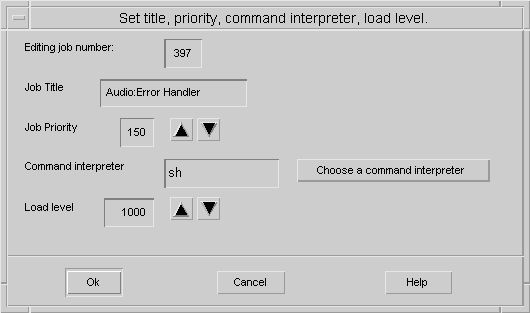
\includegraphics[width=13.877cm,height=8.28cm]{img/ref36.jpg} 

Fields like Priority and Load level take a numeric value which may be typed in or adjusted using the increment and decrement buttons.

Plain text fields like Title simply allow any free text to be entered or modified.

Shown in previous examples are Square buttons which represent options that can be enabled or disabled (true or false). Diamond shape buttons
(not shown in this example) are used for selecting one option out of a set of 2 or more possible options.

Some fields like the Command Interpreter in this example have a Select button next to them. These support two methods of parameter entry,
straight text entry as in the Title field or by selecting one option from a list using a selection dialog. Clicking on the
``Choose a command interpreter'' button, for example, opens this selection dialog.

 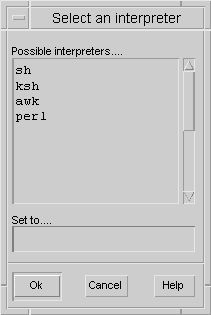
\includegraphics[width=5.525cm,height=8.333cm]{img/ref37.jpg} 

The information displayed is context and configuration sensitive, showing only the permitted and/or appropriate information.

This type of selection dialog does not insert multiple selections or pattern matching characters. However you can select an item from the
list then type other information afterwards.

\section{\XmbtrName{} - Motif Batch Job Submission \& Editing Tool}
Used for creating, editing and submitting batch jobs, \PrXmbtr{} is a GUI alternative to the command line program \BtrName. It provides all of the same options using the Graphical User Interface instead of command line options. It may also be used to edit the default options which both \PrXmbtr{} and
\PrBtr{} read from the current and home directories.

\PrXmbtr{} can edit existing jobs that have been unqueued using \PrBtq{}, \PrXmbtq{} and \PrBtjdel{}. Apart from submitting jobs to the
queue \PrXmbtr{} also saves them in the same ``unqueued job'' format. This uses two files, which are:

Command file

Which is a shell script that holds the specification for the job. This shell script contains statements to reproduce the job environment
followed by a \PrBtr{} command. The \PrBtr{} command has options to set up all of the job
parameters and references the \textit{job file} by name.

Job file

Which contains the text, or script, of the job that is piped into the ``command interpreter'' by the scheduler.

A list of one or more jobs can be held by \PrXmbtr{} at the same time. This is particularly useful when creating a group, or
schedule, of related jobs.

\subsection{Options}
Options to \PrXmbtr{} are saved to the file \homeconfigpath{} off the user's home directory with appropriate keywords.
The user no longer needs to be concerned with resource settings.

\subsection{The Main Window}
When \PrXmbtr{} is invoked the main window will be displayed. By default it will look something like this:

 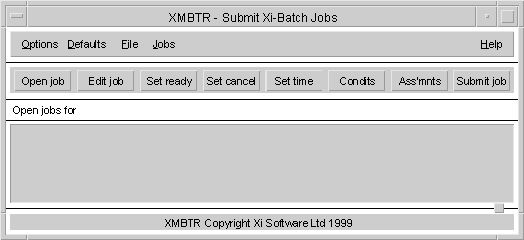
\includegraphics[width=13.72cm,height=6.346cm]{img/ref38.jpg}

The main screen is divided into two key functional areas. The top area contains menus and short cut buttons for issuing commands. The bottom
area displays the list of batch jobs which are being worked on.

\PrXmbtr{} uses similar windows and dialogs to \PrXmbtq{} for specifying the job options.

To edit job scripts \PrXmbtr{} invokes an editor of the user's choice. The editor is specified as a default parameter in the \PrXmbtr{} options. On
installation the default editor is \progname{vi}.

The main screen has a row of menu buttons at the top, underneath of which is a row of short cut buttons. The bottom half of the window is a
scrollable list of the jobs currently being worked on by \PrXmbtr{}.

 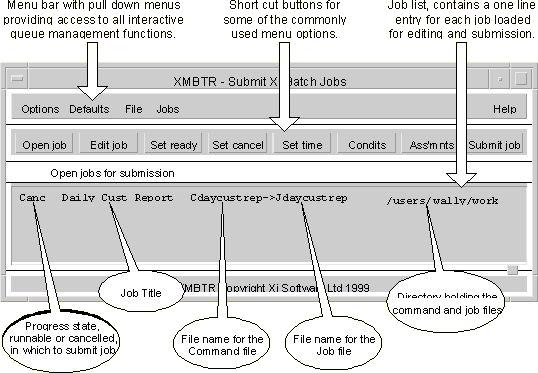
\includegraphics[width=14.085cm,height=9.865cm]{img/ref39.jpg} 

The bubbles in the above picture indicate what each field within a job entry represents.

\subsection{The Menus and Shortcut Buttons}
All commands are performed by selecting a menu option or clicking on the equivalent shortcut button. Some of the menu options may also be
selected using shortcut keys, which are indicated to the right of the relevant options in each menu.

\subsubsection{The Options Menu}
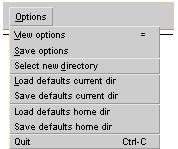
\includegraphics[width=4.657cm,height=3.941cm]{img/ref40.jpg}

For tailoring the look and feel of \PrXmbtr{}, saving the tailored settings, viewing the error log and quitting.

\textbf{View options} brings up the dialog, to specify which text editor to use and whether it should be run inside an X-Terminal session or not.

\textbf{Save options} creates a local copy of the View options.

\textbf{Select new directory} for new jobs to be created in and for getting existing job files from.

\textbf{Load defaults current dir} reads any \XmbtrName{} default settings from the currently set directory.

\textbf{Save defaults current dir} saves the current \XmbtrName{} default settings in the currently set directory.

\textbf{Load defaults home dir} reads any \XmbtrName{} default settings from the user's home directory.

\textbf{Save defaults home dir} saves the current \XmbtrName{} default settings in the user's home directory. \textbf{Quit} terminates
\PrXmbtr{}.

\subsubsection[The Defaults Menu]{The Defaults Menu}
 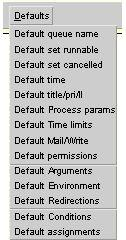
\includegraphics[width=3.297cm,height=6.346cm]{img/ref41.jpg}

For specifying default options for all new jobs being created in this \PrXmbtr{} session.

\textbf{Default queue name} Opens dialog to specify defaults for queue
name, user name and Unix group.

\textbf{Default set runnable} state for jobs.

\textbf{Default set cancelled} state for jobs.

\textbf{Default time} Opens the standard job time and repeat
specification dialog for setting default values.

\textbf{Default title/pri/ll} Opens the standard ``title, priority, command interpreter and load level'' dialog for setting default values.

\textbf{Default Process params} Opens the standard dialog for setting the process parameters: working directory,
\progname{ulimit}, \progname{umask}, exit code ranges, advance time on error flag.

\textbf{Default Time limits} for detecting and stopping over running jobs.

\textbf{Default Mail/Write} job completion flags.

\textbf{Default permissions} for job access modes.

\textbf{Default Arguments} Opens standard dialog for specifying job arguments as defaults.

\textbf{Default Environment} Opens dialog for specifying a default job environment.

\textbf{Default Redirections} Opens standard dialog for specifying job I/O redirections as defaults.

\textbf{Default Conditions} Opens standard dialog for specifying job conditions as defaults.

\textbf{Default assignments} Opens standard dialog for specifying job assignments as defaults.

\subsubsection{The File Menu \& Buttons}
 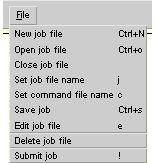
\includegraphics[width=4.082cm,height=4.313cm]{img/ref42.jpg}

Provides options for Submitting jobs, Creating, Editing and Deleting job files.

\textbf{New job file} creates a new, blank entry in the \XmbtrName{} job list. Once created the \textbf{Set command file name}
and \textbf{Set job file name} menu options must be used before a job can be submitted or saved.

\textbf{Open job file} opens a previously saved or unqueued job for editing by \PrXmbtr{}.

\textbf{Close job file} closes both the command file and the job file, then removes the entry from the \PrXmbtr{} display.

\textbf{Set job file name}  opens a file selector dialog for specifying the name of the job file.

\textbf{Set command file name} opens a file selector dialog for specifying the name of the command file.

\textbf{Save job} as 2 files: a command file containing the specification and a job file containing the script.

\textbf{Edit job} file containing the script.

\textbf{Delete job} files and \PrXmbtr{} entry for the job which is currently selected from both the display.

\textbf{Submit job} which is currently selected to the scheduler.

\subsubsection{The Jobs Menu and Buttons}
 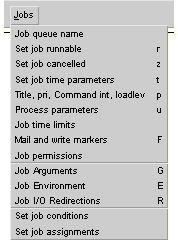
\includegraphics[width=4.657cm,height=6.346cm]{img/ref43.jpg} 

Menu options for specifying the various job parameters.

\textbf{Job queue name} Opens dialog to specify the queue name, user name and Unix group.

\textbf{Set job runnable} This option is also available via the \textbf{Set ready} short cut button.

\textbf{Set job cancelled} This option is also available via the \textbf{Set cancel} short cut button.

\textbf{Set job time parameters} Opens the standard job time and repeat specification dialog.

\textbf{Title, pri, Command int, loadlev} brings up a dialog to specify the Job Title, Priority, Command Interpreter and Load Level.

\textbf{Process Parameters} Opens the standard dialog for setting the process parameters: working directory, ulimit, umask, exit code ranges,
advance time on error flag.

\textbf{Job time limits} opens dialog to set parameters for detecting and stopping over running jobs.

\textbf{Mail and write markers} opens dialog for setting job completion mail and write flags.

\textbf{Job permissions} for access modes. I.e. read, write, etc.

\textbf{Job Arguments} Opens standard dialog for specifying arguments to be passed to the job.

\textbf{Job Environment} Opens dialog for the job environment variables.

\textbf{Job I/O Redirections} Opens standard dialog for specifying job I/O redirections.

\textbf{Set job conditions} Opens standard dialog for specifying job conditions.

\textbf{Set job assignments} Opens standard dialog for specifying job assignments.

\subsubsection{Help}
 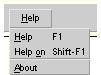
\includegraphics[width=2.641cm,height=1.983cm]{img/ref44.jpg} 

Context sensitive help for using \PrXmbtr{}.

\textbf{Help} displays help for the current window.

\textbf{Help on} changes the operating mode from taking commands to displaying help on any object (menu, button etc.) that is selected.

\textbf{About} displays information, such as release number, about the version of \XmbtrName{} that is running.

\subsection{Choosing a Directory}
By default \PrXmbtr{} will create new jobs and look for existing ones in the Current Working Directory when it was invoked.
This can be changed to a new directory at any time by the \textbf{Select new directory} option under the \textbf{Options} menu.

This opens the standard dialog for selecting directories and files. Change to the required directory and click on OK. There is no need to
specify a file name.

\subsection{Creating a New Job}
There are four essential operations required to create a new job. The first three are probably best done in sequence. This avoids \XmbtrName{}
generating reminder messages later when it needs information from these operations. All of the operations are selected from the File menu as
follows:

 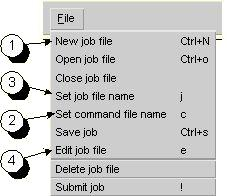
\includegraphics[width=5.943cm,height=5.186cm]{img/ref45.jpg} 

\begin{enumerate}
\item Select the \textbf{New job file} option, which produces a new entry line in the job list. Select this line, if it is not highlighted,
by clicking on it.
\item Use the \textbf{Set command file name} option, to specify a name for the command file. A \textit{Motif}file selection dialog will appear
showing the contents of the current directory. Select a new file name. An alternative directory for the command file can also be specified in
this dialog.

When this is done, the file name will appear in front of the \exampletext{{}-{\textgreater}} symbol on the selected entry
in the job list.
\item Specify a name for the job file, by selecting \textbf{Set job file name} option. A similar \textit{Motif}file selection dialog will
appear, which is used to enter the file (and possibly path) in the same way as for the command file name.

The job file name will appear to the right of the \exampletext{{}-{\textgreater}} symbol this time.
\item It is now possible to create and edit the job script. Select the job by clicking on its entry in the job list and use the \textbf{Edit
job file} option to invoke the text editor. The text editor is automatically loaded with the script for editing - in this case a blank
file.

There are no constraints on when or how many times the script may be edited, once the first three steps have been done.
\end{enumerate}
When a new job is created it will be given a specification based on whatever default options are currently in force. These can include:
queue name, job title and initial state which will be shown on the job list entry. Other settings can only be seen by opening the relevant
specification dialogs, for example \textbf{Set times for job}.

\subsection{Loading an Unqueued or Previously Saved Job}
Use the \textbf{Open jobfile} option from the \textbf{File} menu to open a previously saved or unqueued job. This opens the standard Motif file
selector dialog, in the currently set directory. The file list in the dialog is restricted to show only the Command files of each job. The
dialog can be fooled by files which look like but are not valid command files. This is not dangerous, an error message will be displayed and
another file can be selected.

Select the required job and click on OK. This loads the job specification into \XmbtrName{} and places an entry in the job list.

\subsection{Setting up or Editing the Job Specification}
Select the job by clicking on its entry in the job list. Any of the parameters in the selected jobs specification can now be edited using
the options under the \textbf{Jobs} menu. This menu has a set of options almost identical to those in \PrXmbtq{}.
There are also shortcut buttons for some of these options.

\subsection{Editing the Job Script}
Select the job by clicking on its entry in the job list and use the \textbf{Edit job file} option from the \textbf{File} menu to invoke the
text editor. The text editor is automatically loaded with the script for editing. Alternatively click on the \textbf{Edit job} short cut
button instead of using the menu option.

Change the script, then save the changes and exit as appropriate for the editor. When this is done it is a good idea to save away the command
file as well by selecting the \textbf{Save job} option from the \textbf{File} Menu.

\subsection{Selecting a different Text Editor}
By default \PrXmbtr{} is shipped set up to run the \progname{vi} editor inside an X-Terminal session. This can
be changed to any suitable editor of the user's choice.

Select \textbf{View options} from the \textbf{Options} menu to open the Display options dialog. Type in the name of the desired editor, over
the top of the existing name. If the editor has a Graphical User Interface then un-check the Run editor in
``xterm'' check-box. Otherwise make sure the box is checked to launch a terminal to run the editor.

\subsection{Submitting Jobs}
Jobs can be submitted by selecting their entry in the job list and clicking on the \textbf{Submit job} shortcut button, or by using the
\textbf{Submit job} option from the \textbf{File} menu.

Jobs that have been submitted can be edited to produce other jobs and submitted again, as many times as required. If the job has not been
changed before being submitted again \PrXmbtr{} asks for confirmation.

\subsection{Saving, Closing and Deleting Jobs}
Jobs can be saved at any time. This saves the current specification of the job and leaves it open for further work.

Closing the job removes it from the job list. To avoid losing any changes save the job before closing it.

Deleting a job closes it and deletes the command and job files from the disk.

\subsection{Specifying Defaults}
The same default options as used by \PrBtr{}, are loaded when \PrXmbtr{} is started. The defaults are
read from any \filename{\BtrVarname} keyword entries in relevant \configurationfile{} or \homeconfigpath{} files and the \filename{\BtrVarname}
environment variable if defined. These defaults are applied to any new jobs created in the \PrXmbtr{} session.

The options under the \textbf{Defaults} menu enable the default options to be specified in the same way as the \textbf{Jobs} menu options
change those for individual jobs.

Changes to the default settings can be saved using in the current or user's home directory. This is done using the \textbf{Save defaults current dir} and \textbf{Save defaults home dir} options from the \textbf{Options} menu.

A different set of, or the original, defaults can be loaded from a new directory or from the home directory. This is done using the
\textbf{Select new directory} and \textbf{Load defaults ...} options from the \textbf{Options} menu.

\section{\XmbtuserName{} - Motif GUI User Administration Tool}
\PrXmbtuser{} is a fully interactive Motif alternative to the standard user permission manager (invoked using the command
\PrBtuser{} with option \exampletext{-i}.
It is provided to maintain the list of user privileges and default modes for both jobs submitted
and variables created.

Unlike \PrBtuser{} there are no command line options to \PrXmbtuser{}, it is always in the interactive
mode (similar to \PrBtuser{} with option \exampletext{-i}). The facility to change or specify resource settings for an X11 (and hence Motif)
program on the command line can be used.

A list of user names or patterns for matching user names can be specified. This will restrict the display to the selected users, in the
same way as restricting the display of programs like \PrBtq{}.

\subsection{Options}
It is not necessary to provide options via the resource files any more like with previous versions
of \PrXmbtuser{} as the options selected within the program are automatically saved in the configuration
file \homeconfigpath{} off the user's home directory on request.
\subsection{The Main Window}
When \PrXmbtuser{} is invoked the main window will be displayed. By default it will look something like this:

 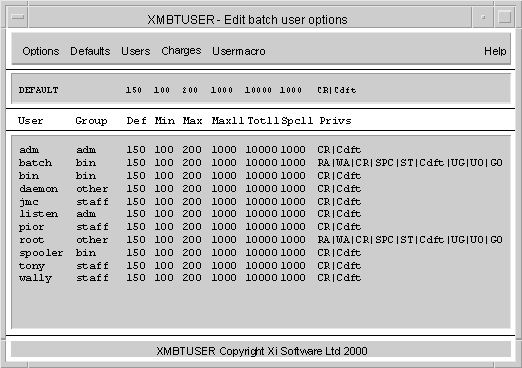
\includegraphics[width=13.667cm,height=9.737cm]{img/ref46.jpg} 

The bottom area contains a list of all users in the password file with their \ProductName{} permissions and settings. It will have a scroll bar if
there are more users than can fit on the screen. Above this is a pane containing the default settings.

At the top of the screen is the menu bar supporting all of the \PrXmbtuser{} commands. Each menu option opens a
dialog or operates on the specified data immediately. With a few exceptions these are straight forward and easy to understand.

\subsection{The Menus and Options}
All commands are performed by selecting a menu option. Some of the menu options may also be selected using shortcut keys, which are indicated
to the right of the relevant options in each menu.

\subsubsection{The Options Menu}
 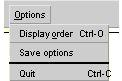
\includegraphics[width=3.193cm,height=2.14cm]{img/ref47.jpg}

For changing the ordering of users in the display, saving the settings and quitting.

\textbf{Display order} brings up the Display options dialog, to tailor the look and feel. Pressing the Control and O keys also invokes this
option.

\textbf{Save options} creates a local copy of the Display order.

\textbf{Quit} saves any changes to the default and user accounts. (N.B. It is at this point that all changes are saved).

\subsubsection{The Defaults Menu}
 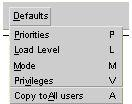
\includegraphics[width=3.454cm,height=2.752cm]{img/ref48.jpg} 

Administers the default account parameters.

\textbf{Priorities} opens the dialog for setting up the maximum, minimum and default priorities for the user(s).

\textbf{Load Level} opens the load level specification dialog. This sets the following:

\begin{itemize}
\item Maximum load level permitted for any one job submitted by the user
\item Maximum number of jobs measured in load that the user may have running at any time
\item A default value for load level for the user if they have \textit{special create} privilege.
\end{itemize}
\textbf{Mode} brings up a dialog for setting the default access modes on all jobs submitted and variables created by the user.

\textbf{Privileges} opens a dialog showing and allowing changes to the privileges (e.g. submit jobs and create variables).

\textbf{Copy to all users} Copies the default settings to all users - \textit{use with care}.

\subsubsection{The Users Menu}
 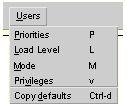
\includegraphics[width=3.321cm,height=2.752cm]{img/ref49.jpg} 

Administers the accounts of individual users

\textbf{Priorities} opens the dialog for setting up the maximum, minimum and default priorities for the user(s).

\textbf{Load Level} opens the load level specification dialog. This sets the following:

\begin{itemize}
\item Maximum load level permitted for any one job submitted by the user
\item Maximum number of jobs measured in load that the user may have running at any time.
\item A default value for load level for the user if they have \textit{special create} privilege.
\end{itemize}
\textbf{Mode} brings up a dialog for setting the default access modes on all jobs submitted and variables created by the user.

\textbf{Privileges} opens a dialog showing and allowing changes to the privileges (e.g. submit jobs and create variables).

\textbf{Copy defaults} resets the users account to the default settings - \textit{use with care}!

\subsubsection{The Usermacro Menu}
 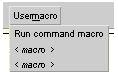
\includegraphics[width=3.089cm,height=1.901cm]{img/ref51.jpg} 

Provides macro commands for use on the selected users.

\textbf{Run command macro} opens a dialog prompting for the name of the macro to run. This is then invoked by \PrXmbtuser{}
with the name(s)of the selected user(s).

\textbf{{\textless} }\textbf{\textit{macro}}\textbf{ {\textgreater}} runs the pre-defined macro, whose name or a brief description will
appear in place of the {\textless} \textit{macro} {\textgreater} place holder.

Up to 9 macros may be pre-defined.

\subsubsection{The Help Menu}
 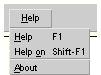
\includegraphics[width=2.641cm,height=1.983cm]{img/ref52.jpg} 

Context sensitive help for using \PrXmbtuser{}.

\textbf{Help} displays help for the current window.

\textbf{Help on} changes the operating mode from taking commands to displaying help on any object (menu, button etc.) that is selected.

\textbf{About} displays information, such as release number, about the version of \PrXmbtuser{} that is running.

\subsection{Selecting multiple users for menu options}
Many of the menu options can be carried out on more than one user at a time. First select all of the relevant users from the list. Then select
the required menu option for the operation you wish to perform. The set of users remains selected after you have completed the operation in
case there are other options that you want to use on them.

You can scroll up and down a long list of users without losing those you have selected so far. The following mechanisms allow you to select a
group of users:

\begin{itemize}
\item Hold the selection mouse button down and drag it across a contiguous set of users.
\item Using the mouse click on the first user in the required set. Move to the last user in the set , hold the shift key down on the keyboard
and click on this user.
\item Individual users may be added or removed from the set by clicking on them whilst holding the Control key down on the keyboard.
\end{itemize}
\subsection{Copying defaults to all users}
Available via the \textbf{Copy to all users} option under the \textbf{Defaults} menu. It copies the default settings to all users
except the one you are logged in as.

This command should be used with care. It is possible to remove essential permissions from everybody including write administration
file privilege (although attempts to deprive \filename{root} and \batchuser{} of these permissions will be silently ignored).

\subsection{Resetting a user to the default}
This is a very useful mechanism for setting permissions for a group of users. Set the default to the required value then apply it to the
required users. If you do not want new users to inherit this default setting remember to return it to the original state.

Note that attempts to deprive \filename{root} and \batchuser{} of full permissions will be silently ignored

\section{\XmfilemonName{} - Optional Motif GUI Interface to \BtfilemonName}
\PrXmfilemon{} provides a simple interface to \PrBtfilemon. It provides a single dialog box of options to invoke \PrBtfilemon{} with.

